\title{Chapter 4, Section 2. Exercises 1, 2, and 4 through 9}
\author{
	MTH 594, Prof. Mikael Vejdemo-Johansson \\
	Differential Geometry Independent Study \\
	\\
	Matthew Connelly \\
}
\date{\today}



\documentclass[12pt]{article}

\usepackage[top=.5in, bottom=.75in, left=1in, right=1in]{geometry}
\usepackage{amssymb}
\usepackage{amsmath}
\usepackage{graphicx}
\usepackage{subcaption}


\begin{document}
\maketitle

\section*{Exercise 4.2.2}
Verify that the six surface patches for $S^2$ in Exercise 4.1.2 are regular. Calculate the transition maps between them and verify that these maps are smooth.

\vspace{1cm}
\hrule
\vspace{1cm}
\noindent
\underline{Preliminary definitions and clarification:}\\\\
This problem is referring to surface $S^2$, which is a sphere that has been split into six \\ surface patches that look like domes. Only two of these patches would be needed to complete the \emph{image} of the surface (but not the surface in its entirety). The parametrization $\sigma$ maps $u,v \in U$ to $S^2 \cap W$ by the following definition:
$$
\sigma^{x}_{\pm}(u,v) = (\pm \sqrt{1-u^2-v^2}, u ,v)
$$
\indent
A near-identical definition is used for the $\pm y$ and $\pm z$ patches.\\
\indent
All six patches can be visualized as the following four domes (or even the just the first two) depicted below through the appropriate rotation/orientation:
\begin{figure}[h!]
  \centering
      \begin{subfigure}[b]{0.5\linewidth}
    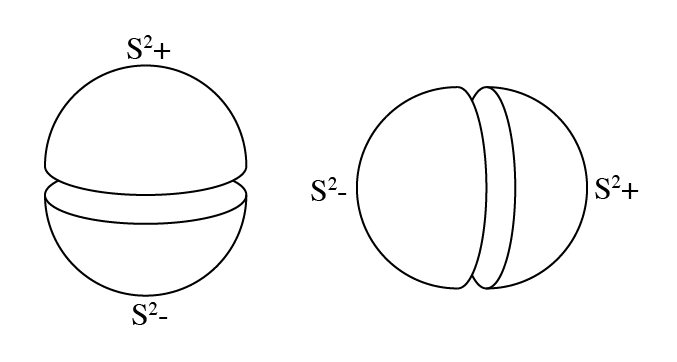
\includegraphics[width=\linewidth]{./assets/4-2-2/s2-patches.png}
  \end{subfigure}
  \end{figure}
  \\
	\indent
	These six patches (four of which could be depicted as above) are essentially nested, creating an overlap between all six and covering the open bounds of each other (covering the edge made by the "slice"), making an atlas for the entirety of $S^2$.

\clearpage

\underline{Verifying regularity of $\sigma$:}\\\\
\indent
We will work with a single surface patch $\sigma^x_+$ and trust that its regularity will imply the regularity of the remaining five patches, considering their near-identical definitions.\\
\indent
We will also take the liberty of taking $\sigma$ to mean $\sigma^x_+$  from here on out for ease of notation.\\\\
\indent
By definition, a surface patch is regular if it is smooth (belonging to $C^n$) and the vectors are linearly independent in the $\mathbb{R}^2$ set to which it is homeomorphic.\\
\indent
Partial differentiation will show that  $\sigma \in C^n$, and is therefore smooth:
$$
\sigma_u = \left(-\frac{u}{\sqrt{1-u^2-v^2}}, 1 ,0 \right)
$$

$$
\sigma_v = \left(-\frac{v}{\sqrt{1-u^2-v^2}}, 0 ,1 \right)
$$
\indent
$U$ can then be defined as:
$$
U = \lbrace u,v \in \mathbb{R}^2 \ | \ u^2 + v^2 < 1 \rbrace
$$
\indent
Letting vectors $u, v \in U$ be orthogonal to each other, and therefore linearly independent, satisfies the final condition that make $\sigma$ regular.\\\\

\underline{Calculating the transition maps between $\sigma$ patches:}\\
\indent

Just as we used a single patch for verifying regularity earlier, we need only work with two patches of $S^2$'s atlas to calculate a transition map between any two of its patches, on account of its symmetry.\\

Let us take the $+x$ and $+z$ patches, then. These patches will be parametrized as the following homeomorphisms:

$$
\sigma^{x}_{+}(u,v) = (\sqrt{1-u^2-v^2}, u ,v)
$$
$$
\sigma^{z}_{+}(u,v) = (u ,v, \sqrt{1-u^2-v^2})
$$

Each of which have the following mappings:

$$
\sigma^{x}_{+} : U \rightarrow S \cap W
$$
$$
\sigma^{z}_{+} : \widetilde{U} \rightarrow S \cap \widetilde{W}
$$

\clearpage

We can visualize $+x$ and $+z$ as the diagram below:

\begin{figure}[h!]
  \centering
      \begin{subfigure}[b]{0.3\linewidth}
    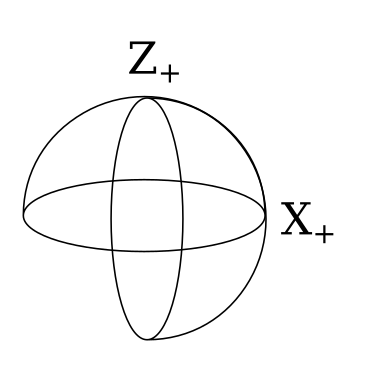
\includegraphics[width=\linewidth]{./assets/4-2-2/s2-patches-intersection.png}
  \end{subfigure}
  \end{figure}
	\indent

The overlap (intersection) of the patches can be written as
$$
\lbrace \sigma^{x}_{+}(u,v)  \ \forall \ (u, v) \in U  \ | \ -2\pi \leq u \leq 2\pi  \ \textrm{and} \ 0 \leq v \leq 2\pi  \rbrace
$$
\indent
or
$$
\lbrace \sigma^{z}_{+}(\tilde u, \tilde v)  \ \forall \ (\tilde u, \tilde v) \in \widetilde{U}  \ | \  0 \leq \tilde u \leq 2\pi  \ \textrm{and} \ -2\pi \leq \tilde v \leq 2\pi \rbrace,
$$

each which would be half of a dome (or a quarter of a sphere).\\

\indent
Then, for some $V \subset U$ and $\widetilde V \subset \widetilde U$,
$$
\sigma^{-1}_{x}(S \cap W \cap \widetilde W) = V
$$

\indent
and

$$
\sigma^{-1}_{z}(S \cap W \cap \widetilde W) = \tilde V
$$

where $S \cap W \cap \widetilde W $ marks the overlap/intersection of the two surface patches.\\
\indent
$\therefore$, the transition map will be

$$
\sigma^{-1}_{x}( \ \sigma_{z}(\widetilde V)  \ ) = \sigma^{-1}_{x}(S \cap W \cap \widetilde W) = V
$$

which can be written as the following composition:
$$
\sigma^{-1}_{x} \circ \sigma_{z} : \widetilde V \rightarrow V
$$

which is smooth because, by definition of a surface patch, $\sigma^{-1}_{x}$ and $\sigma^{-1}_{z}$ are smooth.

\end{document}
This is never printed
